% !TEX ROOT = ../ersti.tex
\subsection{Experimentalphysik 1 - Mechanik und Wärmelehre}
\label{ex1}
Die Experimentalphysik 1 (\gls{Ex}) ist eigentlich eine sehr angenehme Vorlesung, um ins erste Semester zu starten, zumindest sofern ihr in der Schule irgendwann mal Physik hattet. Echte Verständnishürden stellen sich gerade im Mechanikteil im Allgemeinen nicht. Im Großen und Ganzen stellt sie einen Schnelldurchlauf durch die Entwicklung der Mechanik dar, von den Anfängen (diese liegen, je nach Prof, zwischen den alten Griechen und Newtons Axiomen) bis zu etwas ausgefeilteren Sachen, die sich aber alle noch im Rahmen des Schulstoffs bewegen sollten. Was diese Vorlesung dennoch von der Schule unterscheidet ist die \emph{Art} der Präsentation, größtenteils frontaler Vortrag, gespickt mit vielen Experimenten (Manchmal durchaus eine Art „Knoff-Hoff-Show“) und sehr viel schneller und mathematischer als ihr das von eurer Lehrerin gewohnt seit. Trotzdem ist dies die Vorlesung mit dem wahrscheinlich größten Unterhaltungswert eurer ganzen Universitätskarriere.

\begin{figure*}[b]
    \centering
    \begin{subfigure}[b]{.18\textwidth}
    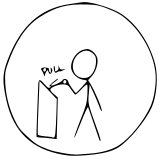
\includegraphics[width=\linewidth]{bilder/the_difference_1.png}	    
    \end{subfigure}
    \begin{subfigure}[b]{.18\textwidth}
    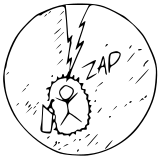
\includegraphics[width=\linewidth]{bilder/the_difference_2.png}
    \end{subfigure}
    \begin{subfigure}[b]{.18\textwidth}
    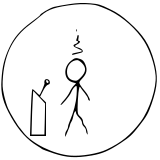
\includegraphics[width=\linewidth]{bilder/the_difference_3.png}
    \end{subfigure}
    \begin{subfigure}[b]{.18\textwidth}
    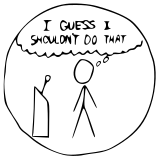
\includegraphics[width=\linewidth]{bilder/the_difference_4A.png}
    \end{subfigure}
    \begin{subfigure}[b]{.18\textwidth}
    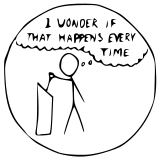
\includegraphics[width=\linewidth]{bilder/the_difference_4B.png}
    \end{subfigure}
\end{figure*}

